\section{ME21B088}

\title{\textbf {Assignment 4} }
\author{\textbf {Khobragade Kashish Vinod me21b088} }
\date{\textbf {June 2022} }

\maketitle

\subsection{Heisenberg Uncertainty Principle}

\subsubsection{Equations}

\begin{equation}
   \Delta x\cdot\Delta p\geq \frac {h}{4\pi}
\end{equation}
  
\begin{equation}
    \Delta x\cdot m\Delta v\geq \frac {h}{4\pi}
\end{equation} 

\begin{equation}
     \Delta E\cdot \Delta t\geq \frac {h}{4\pi}
\end{equation}

\begin{center}
\begin{tabular}{|c|c|}
    \hline
    \textbf{Symbols} & \textbf{Meaning of Symbols} \\
    \hline
    $\Delta x$ & uncertainty in displacement \\
    \hline
    $\Delta p$ & uncertainty in momentum \\
    \hline
    $\Delta v$ & uncertainty in velocity \\
    \hline
    $\Delta E$ & uncertainty in energy \\
    \hline
    $\Delta t$ & uncertainty in time \\
    \hline
    h &  planck's constant value is $\ 6.63*{10}^{-34}$ Jsec \\
    \hline
    m & mass  \\
    \hline
\end{tabular}
\end{center}


According to Heisenberg, it is impossible to measure both the position and momentum of moving particle with accuracy.
 \begin{enumerate}
     \item If value of position is small, it can be measured accurately but not momentum.
     \item If value of momentum is small it is measured accurately but not the position.
 \end{enumerate}
 
 

\subsubsection{Explanation}

\begin{enumerate}
    \item Suppose we need to measure position accurately, then we need to use light.
    \item So, that the photon of light must strike the electron and reflected photon is seen with microscope.
    \item Due to hitting, the position and velocity of electron is changed.
    \item But to pin point position, the light of shorter wavelength should be used.
    \item The shorter wavelength means high frequency and high energy.
    \item So, this high energy photon may change the speed and direction of particle.
\end{enumerate}

\subsubsection{Figure 1}

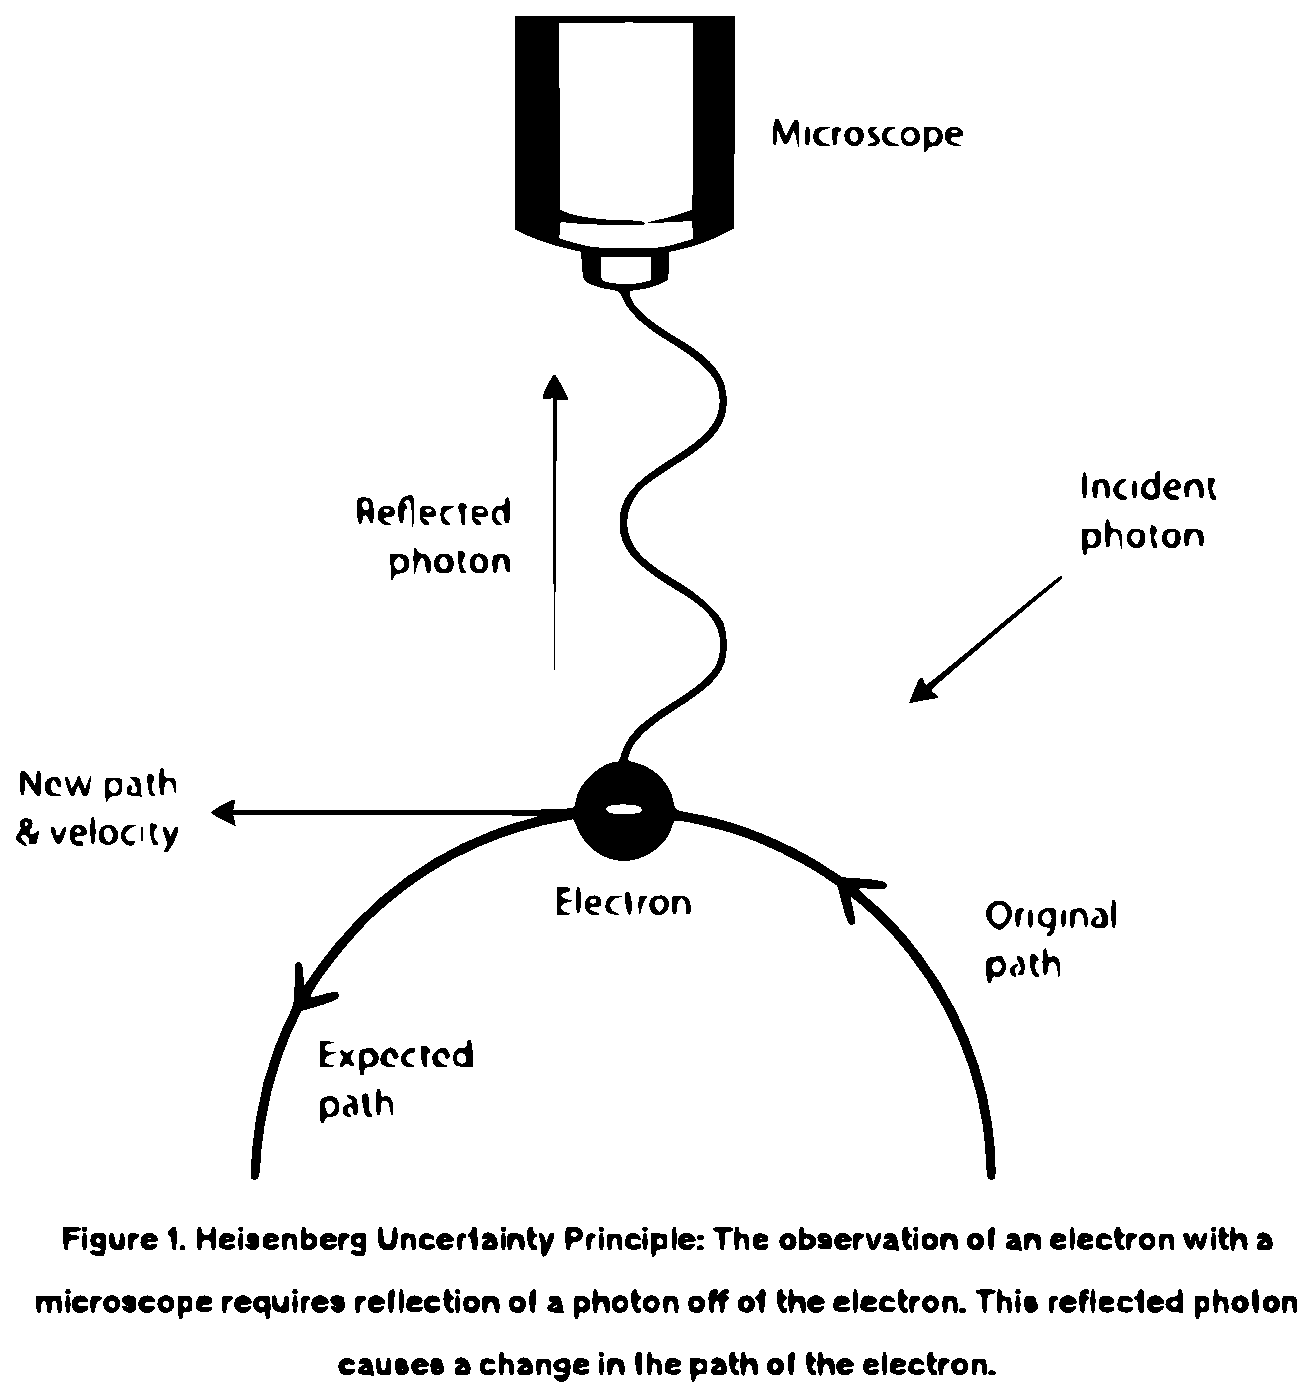
\includegraphics[scale=0.5]{Capture.eps}

\subsubsection{Significance}

This holds good only for microscopic particles, as energy of photon is enough to change the position and velocity of bigger bodies, So, in our daily routine it has no significance.


